\chapter{Introducción a las GUIs MATLAB}

Una interfaz gráfica de usuario (GUI) es un elemento gráfico que
contiene uno o más controles que están disponibles para interactuar con
el usuario mediante un entorno visual sencillo, el cual permite la
comunicación entre el usuario y el computador. Entre algunos de los
componentes más comunes de una GUI creada en MATLAB se tienen menús,
barras de herramientas, botones, menús desplegables, cajas de texto,
entre otros. \\

En las interfaces gráficas creadas en MATLAB pueden aprovecharse todas
las herramientas matemáticas y de ingeniería que proporciona MATLAB,
permiten además la manipulación de archivos de datos, así como la
interacción con otras GUIs y mostrar datos mediante tablas y gráficas de
gran calidad. \\

Generalmente las GUIs son programadas para que respondan a la
manipulación del usuario con una acción específica. Los controles
gráficos que componen una GUI están relacionados con una rutina de
programación, llamada callbacks en el entorno MATLAB, que se ejecuta
cuando sucede un determinado evento, que puede ser la entrada de
caracteres mediante el teclado, el clic de un botón del mouse, o
situarse sobre un objeto. \\

\section{¿Cómo crear una GUI en MATLAB?}

Una interfaz gráfica de usuario en MATLAB puede crearse de dos maneras,
a saber:

\begin{itemize}
\item
  Utilizando el entorno de desarrollo integrado (GUIDE - \emph{Graphical
  User Interface Development Environment}).
\item
  Código puro (programmatically GUI), es decir, utilizando sólo un
  script en el cual se colocarán las instrucciones necesarias para
  producir una interfaz gráfica.
\end{itemize}

¿Cuál es la mejor manera?, imposible dar una respuesta, dependerá mucho
de con cuál el desarrollador se sienta más cómodo. Utilizando GUIDE
puedes desarrollar interfaces gráficas rapidamente, arrastrando
controles y posicionándolos manualmente, para enseguida programar la
lógica principal. Con código puro quizá necesitas un poco más de
\emph{destreza} para colocar y organizar los elementos, pero vamos, nada
complicado en extremo. \\

En este capítulo, para presentar y conocer los objetos gráficos y sus
propiedades utilizaremos código puro, dado que esto permite proporcionar
toda la información necesaria a través del código mostrado, sin requerir
ningún otro tipo de archivo adicional.

\section{Los objetos gráficos en MATLAB}

Los objetos gráficos son los componentes visuales usados por MATLAB para
mostrar información o datos de manera gráfica, a la vez que pueden
permitir que el usuario interactúe mediante diversos controles. \\

Cada objeto tiene un identificador o referencia única llamada
\emph{handle}, mediante el cual se pueden manipular las propiedades del
objeto gráfico. \\

Los objetos gráficos están organizados de manera jerárquica tal como se
muestra en el siguiente diagrama:

\begin{figure}[htbp]
\centering
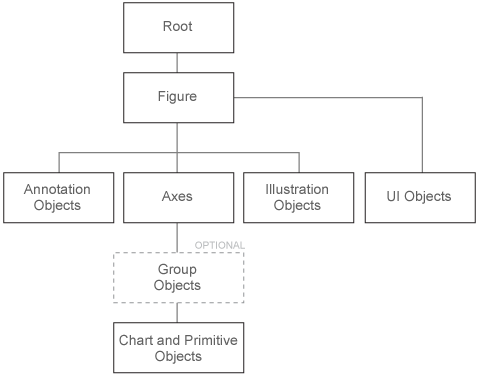
\includegraphics[width=0.6\textwidth]{images/ch8/objetos_graficos.png}
\caption{Jerarquía de los objetos gráficos en MATLAB}
\end{figure}

De manera general, la jerarquía sirve para determinar los objetos que
pueden contener a otro. Un objeto de mayor jerarquía puede contener a
otro de menor rango. Por ejemplo, un axes puede estar contenido dentro
de una ventana o \emph{figure}, viceversa imposible. \\

En el diagrama anterior puede notar que el objeto de mayor jerarquía es
el \emph{Root}, el cual refiere a la base de todo el sistema gráfico de
MATLAB. El objeto \emph{Root} no tiene un objeto padre, pero si puede
tener múltiples \emph{figures} o ventanas como hijos. \\


\begin{informacion}{Objetos padres e hijos}
En este capítulo y en cualquier referencia acerca de
interfaces gráficas encontrará que se hace referencia a
objetos \emph{padres} (\texttt{parent}) y objetos 
\emph{hijos} (\texttt{children}). Por la naturaleza de conceptos es
posible que tenga  una idea acertada de lo que refieren.
Un objeto es \emph{padre} de otro (objeto \emph{hijo}) 
sí este último está contenido dentro del primero. Entender esta relación
es importante,  dado que permita organizar y estructurar
de manera efectiva los controles  gráficos utilizando
\emph{contenedores} (usualmente paneles). Además, debe tomarse
 en cuenta para determinar el \emph{ciclo de vida} de un
objeto gráfico, así, es  pertinente saber que puede
borrar un \emph{hijo} sin afectar al \emph{padre}, pero si borra
 un \emph{padre} estará quitando, también, todos los
objetos que contenga.
\end{informacion}


\section{Propiedades de objetos: funciones \texttt{set} y \texttt{get}}

\section{Objeto \texttt{figure}}

En MATLAB cada interfaz gráfica está creada sobre un objeto
\texttt{figure}, en este elemento se añaden todos los controles gráficos
que componen la GUI. La forma más simple de definir un objeto figure se
ejemplifica enseguida:

\begin{matlab}
hFig = figure;
\end{matlab}

Donde \texttt{hFig} es el handle o referencia del elemento figure.\\

Es muy común que al momento de definir o crear un objeto figure, se
especifiquen algunas de sus propiedades con la sintaxis siguiente:

\begin{matlab}
hFig = figure('Propiedad', 'Valor',...);
\end{matlab}

A continuación se muestra un ejemplo característico:

\begin{matlab}
hFig = figure('NumberTitle','off',...
              'MenuBar','None',...
              'Name','Figure Ejemplo',...
              'Position',[200 200 300 300]);
\end{matlab}

Las propiedades más comunes de un elemento \texttt{figure} se muestran
en la tabla siguiente:

\begin{table}[h!]
\centering
% \rowcolors{1}{}{gray!20}
\begin{tabular}{p{3cm} p{10cm}}
\hline
\Centering\bfseries Propiedad & \Centering\bfseries Descripción \\
\hline
Color & Establece el color de figure. El valor puede establecerse mediante un vector de tres elementos en formato RGB \\
MenuBar & Oculta o muestra la barra de menús estándar de MATLAB \\
Name & Título mostrado en la ventana de la figura. El valor especificado es una cadena de caracteres \\
NumberTitle & Determina si la numeración de los elementos figure creada automáticamente por MATLAB será visible. El valor por defecto es on, para ocultar deberá especificarse off. \\
Position & Especifica el tamaño de la GUI y la posición relativa a la esquina inferior izquierda de la pantalla. El valor se establece mediante un vector de cuatro elementos cuya estructura es la siguiente: [Distancia de la izquierda, Distancia de la parte inferior, Ancho, Alto]; \\
Resize & Determina si puede modificarse el tamaño de la GUI utilizando el mouse. Los valores aceptados son: off y on, siendo este último el valor por defecto. \\
Toolbar & Muestra o borra el menú de herramientas del objeto figure. \\ 
Units & Unidad de medida que se utilizará para interpretar el vector de la propiedad position. Los valores disponibles son: centimeters, characters, inches, normalized, point y pixels. Siendo este último el valor por defecto. \\
Visible & Establece si la GUI es visible. Valores: on y off. \\
\hline
\end{tabular}
\caption{aaaaa}
\end{table}


\section{Controles gráficos (\texttt{uicontrol})}

Los elementos gráficos son todos aquellos componentes que conforman una
interfaz gráfica y que están contenidos dentro de una ventana o
\texttt{figure}. Estos elementos pueden ser campos de texto, botones,
listas desplegables o cualquier otro tipo de elemento gráfico que
permita una interacción con el usuario. \\

En esta sección vamos a ver cómo crear los controles básicos utilizando
la función \texttt{uicontrol}, misma que tiene una sintaxis como sigue:

\begin{matlab}
hCont = uicontrol(Parent, 'Style', 'tipo de control',...
                  'Propiedad', 'Valor');
\end{matlab}

Donde \texttt{Parent} es un objeto gráfico de mayor jerarquía (como
puede ser un panel o un frame/ventana) en el cual va a estar contenido
el control gráfico. La propiedad \texttt{style} define el tipo de
control gráfico a desarrollar. Luego, se pueden pasar varios
\emph{argumentos pareados} o de tipo \texttt{Nombre-Valor}que definan
otras características del control como pueden ser la posición, el color,
el contenido o valor, o bien la asociación a una función que maneje el
evento \emph{disparado} cuando el usuario o la lógica del programa
interaccionen con este. En \texttt{hCont} se guardará la referencia al
objeto creado, mediante la cual posteriormente podemos acceder o
modificar sus propiedades con las funciones \texttt{get} y \texttt{set}. \\ 

En la siguiente tabla se muestran los posibles tipos de control que
pueden ser pasados en la propiedad \texttt{style}.

\begin{table}[h!]
\centering
% \rowcolors{1}{}{gray!20}
\begin{tabular}{p{3cm} P{10cm}}
\hline
\Centering\bfseries Tipo (style) & \Centering\bfseries Control gráfico \\
\hline

checkbox & 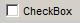
\includegraphics[scale=0.75]{images/ch8/checkbox.png} \\
edit & 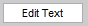
\includegraphics[scale=0.75]{images/ch8/edit.png} \\
listbox & 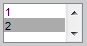
\includegraphics[scale=0.75]{images/ch8/listbox.png} \\
popupmenu & 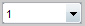
\includegraphics[scale=0.75]{images/ch8/popupmenu.png} \\
pushbutton & 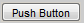
\includegraphics[scale=0.75]{images/ch8/pushbutton.png} \\
radiobutton & 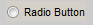
\includegraphics[scale=0.75]{images/ch8/radiobutton.png} \\
slider & 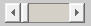
\includegraphics[scale=0.75]{images/ch8/slider.png} \\
text & 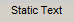
\includegraphics[scale=0.75]{images/ch8/text.png} \\
togglebutton & 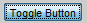
\includegraphics[scale=0.75]{images/ch8/togglebutton.png} \\

\hline
\end{tabular}
\caption{Valores especiales}
\end{table}


La siguiente tabla resume algunas de las \emph{propiedades pareadas} más
utilizadas, que pueden pasarse como argumentos a la función \texttt{uicontrol}:

\begin{table}[h!]
\centering
% \rowcolors{1}{}{gray!20}
\begin{tabular}{p{3cm} p{9cm}}
\hline
\Centering\bfseries Propiedad & \Centering\bfseries Descripción \\
\hline
BackgroundColor & Establece el color del control. El valor puede establecerse mediante un vector de tres elementos en formato RGB. \\

Callback & Función que se ejecuta cuando el usuario interactúa con el control gráfico. El valor pasado puede ser la referencia a una función, por ej: \texttt{@mifuncion} \\

FontName & Fuente a utilizar. Debe ser un string con el nombre de la fuente, la cual debería estar instalada. \\

FontSize & Tamaño de fuente. Valor numérico en las unidades dadas por \texttt{FontUnits} \\

FontUnits & Unidad utilizada para interpretar el valor numérico de \texttt{FontSize} \\

FontWeight & Aspecto de la fuente, puede ser \texttt{normal} o \texttt{bold} (negritas), por default es \texttt{normal} \\

ForegroundColor & Color de la fuente utilizada en control gráfico \\

Parent & Objeto gráfico padre. El valor debe ser un handle o referencia a un objeto gráfico de mayor jerarquía. \\

Position & Especifica el tamaño del control y la posición relativa a la esquina inferior del objeto padre. El valor se establece mediante un vector de cuatro elementos cuya estructura es la siguiente: \texttt{[Distancia de la izquierda, Distancia de la parte inferior, Ancho, Alto]} \\

String & Cadena de texto que se muestra en el control. El valor pasado como argumento puede ser cualquier string. \\ 

Units & Unidad de medida que se utilizará para interpretar el vector de la propiedad \texttt{position}. 
Los valores disponibles son: centimeters, characters, inches, normalized, point y pixels. Siendo este último el valor por
defecto. \\

Visible & Establece si el control es visible. Valores: \texttt{on} y \texttt{off}. \\

\hline
\end{tabular}
\caption{Valores especiales}
\end{table}


\subsection{Check Box}\label{check-box}

El Check Box es un elemento gráfico que sirve como casilla de
verificación, para indicar dos posibles estados: activado/desactivado o
falso/verdadero, como un tipo de check list. Vea el siguiente código:


\begin{matlab}
figure('MenuBar','none',...
    'Position',[100 100 200 100]);

uicontrol('style','checkbox',...
    'string','Rojo',...
    'Position',[10 10 80 20],...
    'Callback',@cambia_color);

    function cambia_color(src, ~)
        if get(src,'Value') == true
            set(gcf,'Color','r');
        else
            set(gcf,'Color',0.8*ones(1,3));
        end
    end
end
\end{matlab}

El código anterior crea una ventana de 200x100 pixeles que contiene un
check box con el string \texttt{Rojo}. Además, puede notar que a la
propiedad \texttt{Callback} se la pasa como argumento una función
\verb|cambia_color| que cada vez que es ``llamada'' cambia el color
de fondo de la ventana: a rojo cuando se activa el check box y al color
por default cuando se desactiva.

\begin{figure}[htbp]
\centering
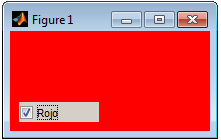
\includegraphics[width=0.4\textwidth]{images/ch8/checkbox_example.png}
\caption{Checkbox}
\end{figure}

\subsection{Edit Text}\label{edit-text}

Un \emph{edit text} es un campo de texto editable en el cual se puede
introducir información en forma de texto, es el clásico \emph{input} que
todos conocemos, como la barra de búsqueda en un buscador de internet o
aquellos cuando rellenamos un formulario \emph{online}.

\subsection{List Box}\label{list-box}

\subsection{Pop-up Menu}\label{pop-up-menu}

\subsection{Push Button}\label{push-button}

\subsection{Radio Button}\label{radio-button}

\subsection{Slider}\label{slider}

\subsection{Static Text}\label{static-text}

\subsection{Toggle Button}\label{toggle-button}


\section{Paneles}\label{paneles}

\section{Axes}\label{axes}

\section{Tablas}\label{tablas}
